% counter has to be defined outside of the frame, otherwise a new counter is created at each iteration of only
\newcounter{slideno}
\begin{frame}{Fibonacci word from above}
(Infinite) Fibonacci word: \ca\cb\ca\ca\cb\ca\cb\ca\ca\cb\ca\ca\cb\dots

\ca{} $\leftrightarrow$ horizontal step, \cb{} $\leftrightarrow$ vertical step

\centering
\forloop{slideno}{1}{\value{slideno} < 14}{%
\only<\theslideno>{\includegraphics[width=.9\textwidth]{img/CP_fibo_\theslideno}}%
}
\end{frame}

\begin{frame}{Quasiperiodicity of the Fibonacci word}
\centering
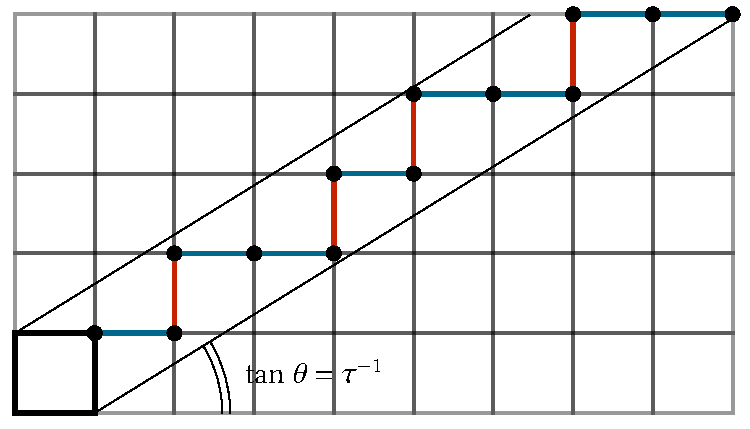
\includegraphics[width=.9\textwidth]{img/CP_fibo_cut}
\end{frame}

\begin{frame}{Cut-and-project}
Quasiperiodic tiling $\Leftrightarrow$ non-periodic tiling constructed with the cut-and-project algorithm.

\(
\<{6cm}
\centering
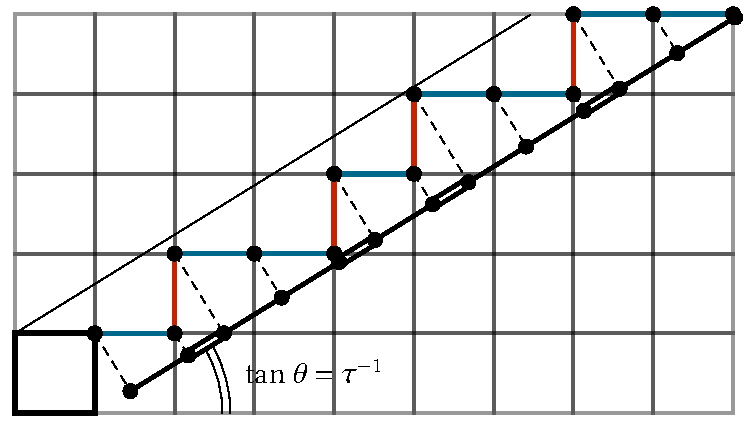
\includegraphics[width=1.\textwidth]{img/full_cp}
\>
\<{6cm}
The cut-and-project algorithm:
\begin{enumerate}
	\item choose a hypercubic lattice (here $\zahl^2$)
	\item choose a ``physical plane'' $E_\parallel$ (here a slope)
	\item select points by translating the unit hypercube along $E_\parallel$
	\item project them onto $E_\parallel$.
\end{enumerate}
\>
\)
\end{frame}

\section{Fractal dimensions}
\subsection{Dummy}
\begin{frame}{Fractal dimensions}
\begin{itemize}
	\item $M(L) \propto L^d$ for a non-fractal $d$-dimensional object\dots What happens for a fractal one?
	
	{\centering
	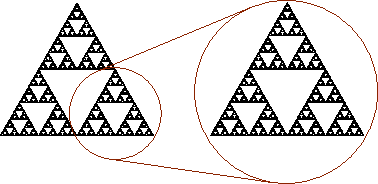
\includegraphics[width=.4\textwidth]{img/sierpinski}
	
	{\ss A Sierpiński triangle}
	
	}
	
	\[
		M(L) \sim L^{d_0} \text{, with } d_0 = \log 3/\log 2
	\]
	
	\item $d_0$ is the Hausdorff fractal dimension
	\item $1 < d_0 \simeq 1.58 < 2$, signature of a fractal object
	\item Probe fractality of the $q^\text{th}$ moment of a distribution $\to$ generalized fractal dimensions $d_q$.
\end{itemize}
\end{frame}

\section{Quantum Fibonacci chain}
\subsection{Dummy}
\begin{frame}{Fractality of the Fibonacci spectrum}
\centering
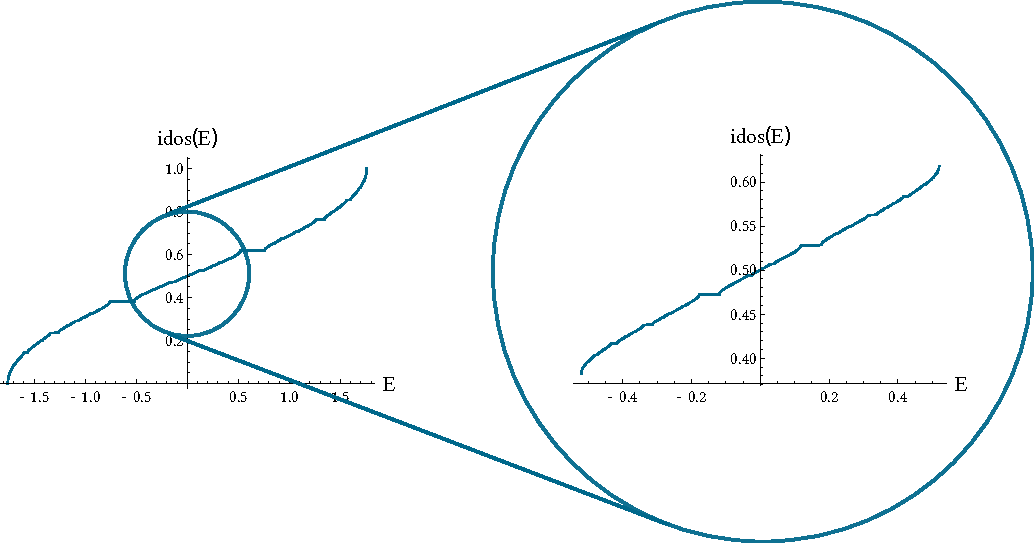
\includegraphics[width=1.\textwidth]{img/idos}	

\flushleft
[Kohmoto \etal{} 89]
\end{frame}

\begin{frame}{Fractality of the $E=0$ eigenstate}
\centering
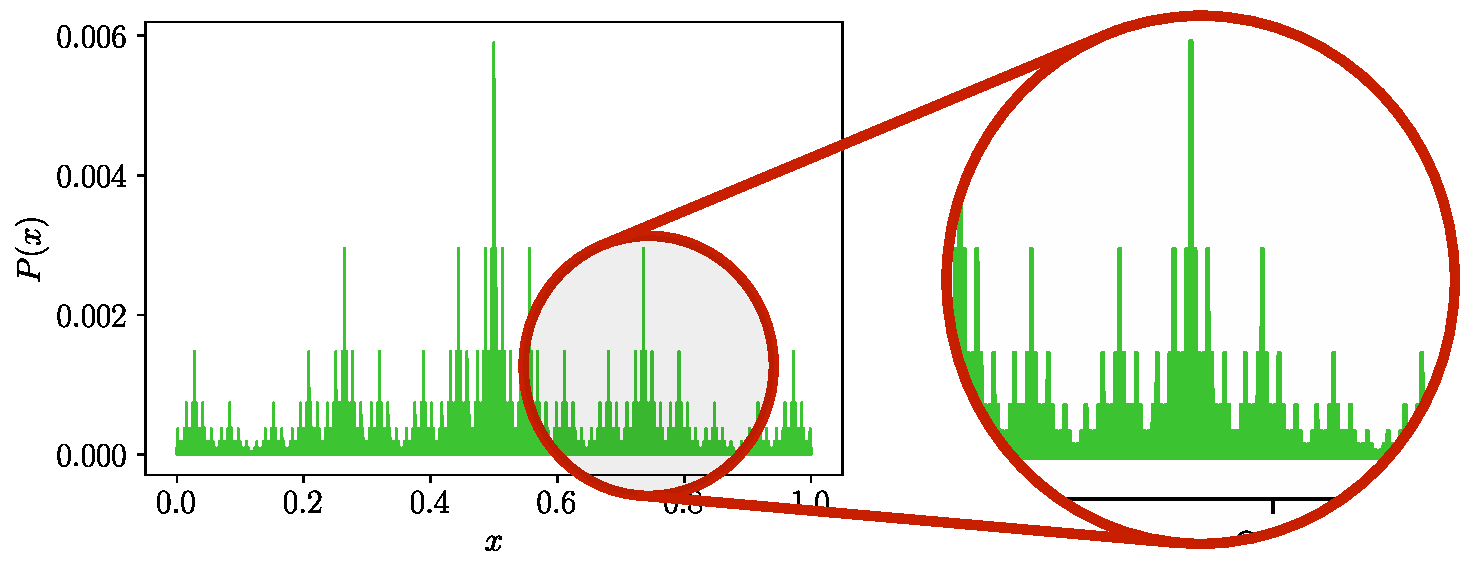
\includegraphics[width=1.\textwidth]{img/fractal_state}

\flushleft
$D_0$ probes the fractality of the tiling:
\[
	D_0 = 1
\]
$D_{q>0}$ probes the fractality of the state:
\[
	0 < D_{q>0} < 1
\]
\end{frame}

\begin{frame}{Height field and state}
\centering
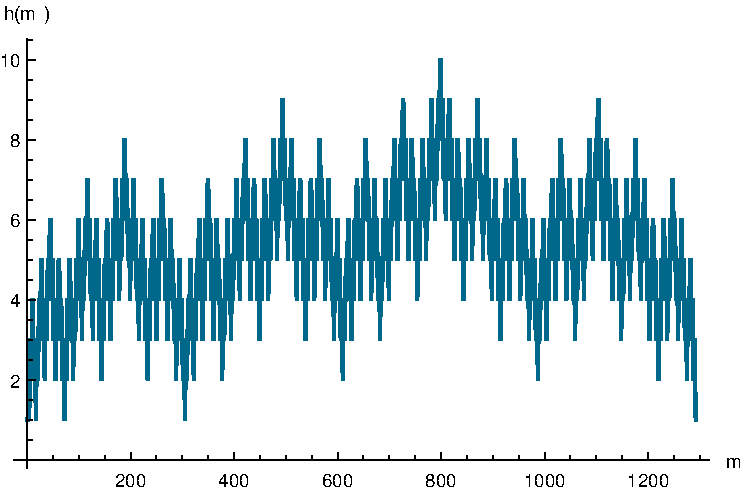
\includegraphics[width=.5\textwidth]{img/heights}

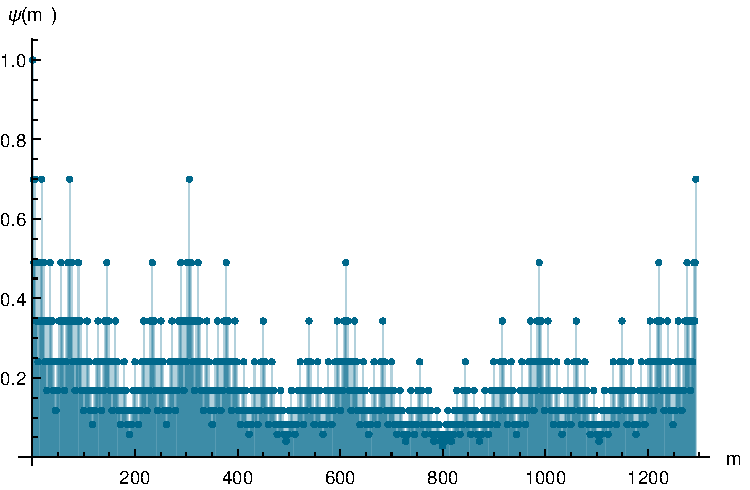
\includegraphics[width=.5\textwidth]{img/wavefunction}
\end{frame}

\begin{frame}{Power-law decay on the Fibonacci chain}
\centering
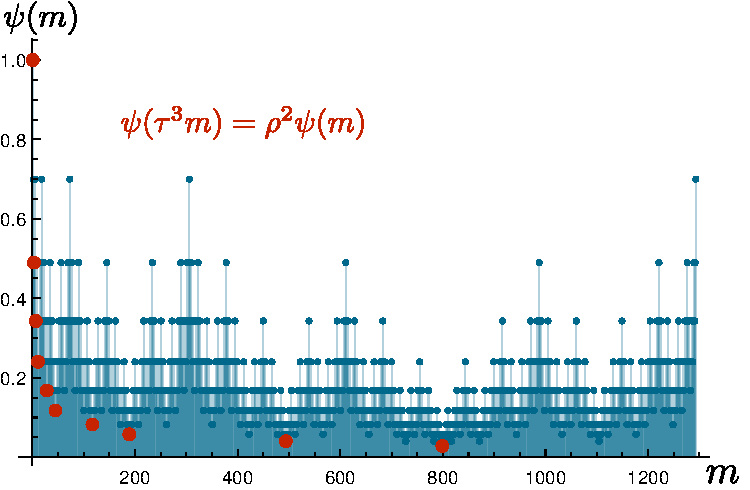
\includegraphics[width=.7\textwidth]{img/power_law_decay}
\end{frame}

%\begin{frame}{Underlying scale invariance}
%Fibonacci chain \emph{itself} scale invariant?
%
%\(
%\<{7cm}
%\begin{itemize}
%	\item Fibonacci words by concatenation:\\
%	$C_2 = \lett{AB}$ \\
%	$C_3 = \lett{ABA}$ \\
%	$C_4 = C_3 C_2 = \lett{ABAAB}$
%	
%	\item Fibonacci words by \textbf{substitution}:
%	\[
%		\sub: 
%		\begin{cases}
%			\A \to \lett{AB}\\
%			\B \to \A.
%		\end{cases}
%	\]
%	$C_3 = \lett{ABA}$ \\
%	$C_4 = S(C_3) = 
%	\only<1>{\sub(\A)\sub(\B)\sub(\A)}
%	\only<2>{\lett{AB}\sub(\B)\sub(\A)}
%	\only<3>{\lett{AB}\A\sub(\A)}
%	\only<4>{\lett{AB}\A\lett{AB}}
%	$
%\end{itemize}
%\>
%\<{7cm}
%\begin{itemize}
%	\item Infinite chain = fixed point of the substitution: \\
%	$S(\lett{ABAAB}\dots) = \lett{ABAAB}\dots$
%	\item Geometric substitution:
%	
%	{\centering
%	    	\begin{tikzpicture}[scale=.6]
    		\newcommand{\orig}{-1.5}
    		\newcommand{\s}{1.5} % length of short bonds
    		\renewcommand{\L}{2.4} % length of long bonds
    		\newcommand{\golden}{1.61}
    		\newcommand{\rs}{\golden*\s} % length of renormalized short bonds
    		\newcommand{\rL}{\golden*\L} % length of renormalized long bonds
    		\newcommand{\vertspac}{2.}    		
    		\newcommand{\rad}{2pt} % radii of the circles
    		\newcommand{\del}{0.2}
    		
    		% set the style of the strong bonds
    		\tikzset{
    			strong/.style={
    				double,
    				double distance=\rad,
    				line width=0.5pt
    				}
    		}
    	
    		%%%%%%%%%% initial chain
    		% bonds 
			\draw[-] (\orig,\vertspac) -- (\orig+\rL,\vertspac) node [midway, below] {$\A$};
			\draw[strong] (\orig+\rL,\vertspac) -- (\orig+\rs+\rL,\vertspac) node [midway, below] {$\B$};	
    		% sites
		    \filldraw (\orig,\vertspac) circle (\rad);% node [below] {6};
		    \filldraw (\orig+\rL,\vertspac) circle (\rad);% node [below] {3};
		    \filldraw (\orig+\rs+\rL,\vertspac) circle (\rad) node [right] {\dots};% node [below] {8};
		        
    		%%%%%%%%% renormalized chain
    		% bonds 
			\draw[-] (\orig,0) -- (\orig+\L,0) node [midway, below] {$\A$};
			\draw[strong] (\orig+\L,0) -- (\orig+\s+\L,0) node [midway, below] {$\B$};	
			\draw[-] (\orig+\s+\L,0) -- (\orig+\s+2*\L,0) node [midway, below] {$\A$};
%			\draw[-] (\orig+2*\s+2*\L,0) -- (\orig+2*\s+3*\L,0) node [midway, below] {$\A$};
%			\draw[strong] (\orig+2*\s+3*\L,0) -- (\orig+3*\s+3*\L,0) node [midway, below] {$\B$};
%			\draw[-] (\orig+3*\s+3*\L,0) -- (\orig+3*\s+4*\L,0) node [midway, below] {$\A$};
%			\draw[strong] (\orig+3*\s+4*\L,0) -- (\orig+4*\s+4*\L,0) node [midway, below] {$\B$};
    	
    		% sites
		    \filldraw (\orig,0) circle (\rad);% node [below] {6};
		    \filldraw (\orig+\L,0) circle (\rad);% node [below] {3};
		    \filldraw (\orig+\s+\L,0) circle (\rad);% node [below] {8};
		    \filldraw (\orig+\s+2*\L,0) circle (\rad) node [right] {\dots};% node [below] {5};
%		    \filldraw (\orig+2*\s+3*\L,0) circle (\rad);% node [below] {2};
%		    \filldraw (\orig+3*\s+3*\L,0) circle (\rad);% node [below] {7};
%		    \filldraw (\orig+3*\s+4*\L,0) circle (\rad);% node [below] {4};
%		    \filldraw (\orig+4*\s+4*\L,0) circle (\rad);% node [below] {1};

		    % arrows below rectangles
		    \draw [<-] (\orig,\del) -- (\orig,\vertspac-\del) node [midway, left] {$\times \frac{1}{\tau}$};
		    \draw [<-] (\orig+\rL,\del) -- (\orig+\rL,\vertspac-\del);
		    \draw [<-] (\orig+\rs+\rL,\del) -- (\orig+\rs+\rL,\vertspac-\del);
		      
		\end{tikzpicture}
%	}
%	
%	\item \textbf{Infinite chain scale invariant}, scaling factor $1/\tau$.
%	
%\end{itemize}
%\>
%\)
%\end{frame}

\begin{frame}{B3 chain and height function}
\(
\<{6cm}
\centering
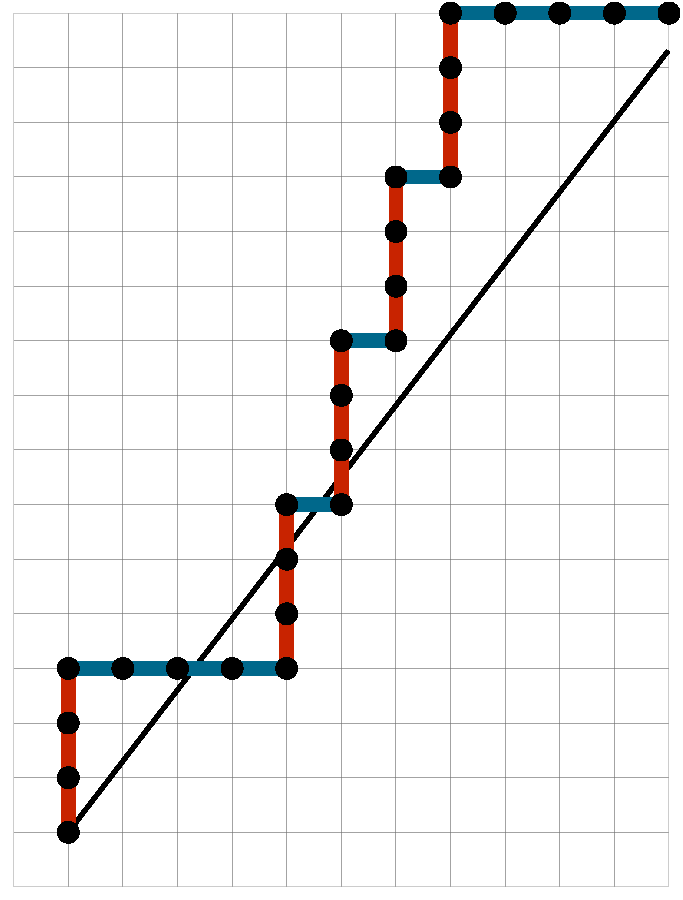
\includegraphics[width=.8\textwidth]{img/CP_b3_cut}
\>

\<{6cm}
\centering
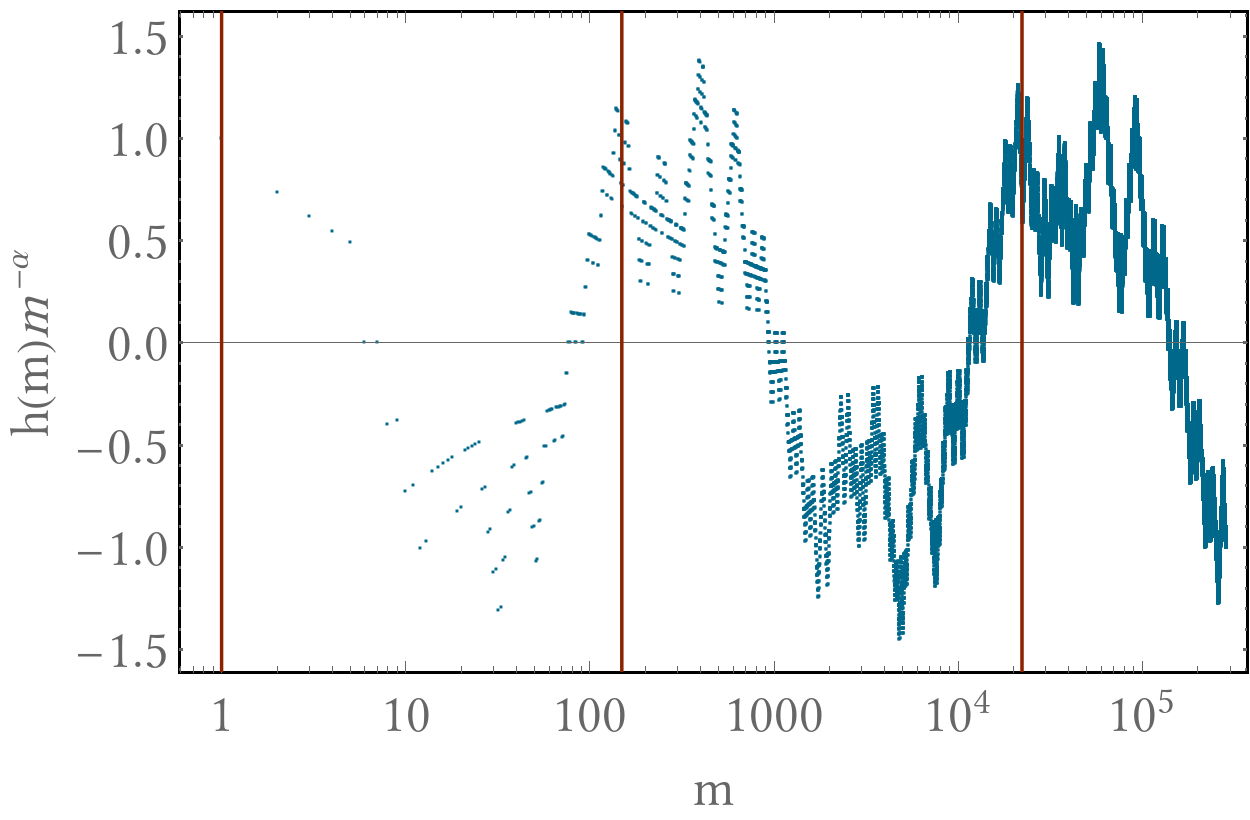
\includegraphics[width=.9\textwidth]{img/height_b3}
\>
\)
\end{frame}